%%%%%%%%%%%%%%%%%%%%%%%%%%%%%%%%%%%%%%%%%%%%%%%%%%%%%%%%%%%%%%%%%%%%%%%%%%%%%%%%
\section{Databases And Capture Methods}\label{ch:bg_db_capture}
%%%%%%%%%%%%%%%%%%%%%%%%%%%%%%%%%%%%%%%%%%%%%%%%%%%%%%%%%%%%%%%%%%%%%%%%%%%%%%%%
In contrast to generic shape recovery, facial shape recovery implies a strong
assumption that the input image contains a face. This prior knowledge, that the
image contains a face, enables the use of training data to improve the
quality of the reconstruction. However, collection of this training data, which
may take the form of either direct 3D information (meshes, range images) or
functions of the facial surface (normals, parametric reflectance data) must
use accurate shape recovery methods in order to be useful. Therefore, the
collection of accurate facial shape for the purposes of providing approximate
ground truth data is a research topic in its own right. In this section, we
begin by discussing the existing 3D facial databases and the manner of their
collection. Following this, we discuss the details of the 3D recovery algorithms
and focus on works intended specifically for facial surface recovery.
%%%%%%%%%%%%%%%%%%%%%%%%%%%%%%%%%%%%%%%%
% CANDIDE 3d wireframe model
% MPI     7 views, 200 laser scanned heads, 5 full 3D, Cyberware, static, neutral
% ND-D    953 scans, Minolta Vivid 900 3D scanner, 656 subjects, neutral, static
% ND-2006 13,450 images containing 6 different types of expressions, 888 distinct people
%         Static, Minolta Vivid 910 range scanner
% 3D-TEC 212 individuals (106 twins),  Minolta VIVID 910 3D scanner, 1 neutral, 1 smiling, static
% CASIA 3D 4624 scans of 123 persons, Minolta Vivid 910, various poses, emotions, static
% B3D(AC)^2 scanned using \cite{weise2007fast}, 14 subjects, 1109 sequences, dynamic 25 FPS, reading
% BIWI Head Pose  15K images of 20 people, various head poses, missing frames, kinect
% UOY Face Database 97 people, multi-pose, neutral, smile and frown
% GavabDB 61 individuals, 427 images, multi pose, static, 3 expressions
% FRAV3D 106 subjects,  MINOLTA VIVID-700, multi-pose, static
% Basel 200 scans, neutral, ABW-3D structured light scanner
% BJUT-3D, cyberware
% EURECOM Kinect, 52 people * 18 image, multi poses, expressions, static
% XM2VTS stereo, 25 subjects, neutral,
% Texas 3DFRD 1149 pairs of facial color and range images of 105 adult human subjects,
%             stereo imaging system manufactured by 3Q Technologies, neutral, frontal
% ZJU-3DFED  40 subjects, total 360, expressions, InSpeck 3D MEGA Capturor DF
% 3D_RMA structured light, 120 people, 6 shots, multi-pose
% Beckmann cyberware, 400-500, single shot
% UMB-DB Minolta Vivid 900 laser scanner
\begin{table}
\centering
\resizebox{\textwidth}{!}{%
\begin{tabular}{@{}lrcccccc@{}}
\toprule
\multicolumn{3}{c}{DB}                                                              & \# Subjects & \# Outputs  & Expressions & Poses & Type   \\ \midrule
CANDIDE v1                  &\cite{Rydfalk:1987tg}          & 1987                  & 1           & 1           & $\cm$       & ---   & MO     \\ \midrule
MPI                         &\cite{Troje:1996ep}            & 1996                  & 200         & 200         &             &       & M      \\ \midrule
CANDIDE v2                  &\cite{Ahlberg:1998uk}          & \multirow{2}{*}{1998} & 1           & 1           & $\cm$       & ---   & MO     \\
3D\_RMA                     &\cite{beumier2001face}         &                       & 120         & 720         &             & $\cm$ & D      \\ \midrule
USF                         &\cite{RefWorks:96}             & \multirow{3}{*}{1999} & 200         & 200         &             & ---   & MO     \\
XM2VTSdb                    &\cite{messer1999xm2vtsdb}      &                       & 295         & 2360        &             &       & M      \\
YaleB                       &\cite{georghiades2001fromfew}  &                       & 10          & 5760        & $\cm$       &       & PS     \\ \midrule
CASIA 3D                    &\cite{casia3d}                 & \multirow{2}{*}{2003} & 123         & 1845        & $\cm$       &       & D      \\
FSU                         &\cite{hesher2003novel}         &                       & 37          & 222         & $\cm$       &       & D      \\ \midrule
GavabDB                     &\cite{moreno2004gavabdb}       & 2004                  & 61          & 720         & $\cm$       & $\cm$ & D      \\ \midrule
FRGC v2                     &\cite{phillips2005overview}    & 2005                  & 466         & 4007        & $\cm$       &       & D      \\ \midrule
BU3D-FE                     &\cite{Yin:2006cc}              & \multirow{4}{*}{2006} & 100         & 2500        & $\cm$       &       & M      \\
ND-2006                     &\cite{faltemier2007using}      &                       & 888         & 13450       & $\cm$       &       & D      \\
FRAV3D                      &\cite{conde2006multimodal}     &                       & 106         & 1696        & $\cm$       &       & M      \\
ZJU-3DFED                   &\cite{wang2006exploring}       &                       & 40          & 360         & $\cm$       &       & M      \\ \midrule
Beckmann                    &\cite{hu2007building}          & 2007                  & $\sim$400   &~?           & $\cm$       &       & M      \\ \midrule
Bosphorus                   &\cite{Savran:2008gg}           & \multirow{3}{*}{2008} & 105         & 4652        & $\cm$       &       & M      \\
UoY                         &\cite{heseltine2008three}      &                       & 350         & 5250        & $\cm$       & $\cm$ & M      \\
BU4D-FE                     &\cite{yin2008high}             &                       & 101         & Many        & $\cm$       & $\cm$ & 4D M   \\ \midrule
Basel                       &\cite{paysan20093d}            & \multirow{2}{*}{2009} & 200         & 200         &             & ---   & MO     \\
BJUT-3D                     &\cite{baocai2009bjut}          &                       & 500         & 500         &             &       & M      \\ \midrule
B3D (AC)\textsuperscript{2} &\cite{fanelli20103}            & \multirow{2}{*}{2010} & 14          & Many        & $\cm$       &       & 4D D/M \\
Texas 3DFRD                 &\cite{gupta2010anthropometric} &                       & 118         & 1149        &             &       & M      \\ \midrule
3D-TEC                      &\cite{vijayan2011twins}        & \multirow{4}{*}{2011} & 212         & 212         & $\cm$       &       & M      \\
BIWI Head Pose              &\cite{fanelli2013random}       &                       & 20          & $\sim$15000 &             & $\cm$ & D      \\
UMB-DB                      &\cite{colombo2011umb}          &                       & 143         & 1473        & $\cm$       &       & M      \\
Florence 3D                 &\cite{bagdanov2011florence}    &                       & 53          & 212         &             & $\cm$ & M      \\ \midrule
ICT-3DRFE                   &\cite{stratou2012exploring}    & \multirow{2}{*}{2012} & 23          & 345         & $\cm$       &       & PS     \\
Superfaces                  &\cite{berretti2012superfaces}  &                       & 20          &~?           &             & $\cm$ & M/D    \\ \midrule
Photoface                   &\cite{RefWorks:293}            & 2013                  & 261         & 1839        & $\cm$       &       & PS/M   \\ \midrule
FaceWarehouse               &\cite{Cao:2014gy}              & \multirow{3}{*}{2014} & 150         & 3000        & $\cm$       & ---   & MO/D   \\
BP4D-Spontaneous            &\cite{Zhang:2014id}            &                       & 41          & Many        & $\cm$       & $\cm$ & 4D M   \\
EURECOM                     &\cite{min2014kinectfacedb}     &                       & 52          & 936         & $\cm$       & $\cm$ & D      \\ \midrule
SURREY                      &\cite{Huber:F5Dca9zy}          & 2016                  & 169         & 169         &             & ---   & MO     \\ \bottomrule
\end{tabular}%
}
\caption{A timeline of existing 3D facial databases (DB) including depth data, mesh
         data, models and Photometric Stereo images. PS denotes Photometric
         Stereo images, MO is a statistical model, M is a 3D mesh,
         D is depth/range data and 4D implies a 3D video.}
\label{tbl:timeline_db}
\end{table}
%%%%%%%%%%%%%%%%%%%%%%%%%%%%%%%%%%%%%%%%
%%%%%%%%%%%%%%%%%%%%%%%%%%%%%%%%%%%%%%%%%%%%%%%%%%%%%%%%%%%%%%%%%%%%%%%%%%%%%%%%
\subsection{Databases}\label{subsec:bg_databases}
%%%%%%%%%%%%%%%%%%%%%%%%%%%%%%%%%%%%%%%%%%%%%%%%%%%%%%%%%%%%%%%%%%%%%%%%%%%%%%%%
The collection of 3D facial databases has a rich history
that spans over many decades. \cref{tbl:timeline_db} provides a
timeline outlining these 3D facial databases and the composition of the
data that they provide.
It is particularly interesting to note that, despite the fact that one of the
first 3D facial models was released in 1987 (CANDIDE~\cite{Rydfalk:1987tg}), the
majority of existing databases were produced in the last decade. The quality
of these facial models has also increased substantially, which is demonstrated
in \cref{fig:db_examples}.

The CANDIDE~\cite{Rydfalk:1987tg,Ahlberg:1998uk} models were parametrizable
wireframe models that contained a low number of vertices (75--95) and were
designed to be controlled according to pre-defined Action Units. The CANDIDE
model was not captured from real data and thus had limited uses for modelling
identity. Early attempts at recording facial databases focused on the use
of laser scanning technology~\cite{cyberware,minolta} or structured light. For
example, the early work of \citet{beumier2001face} used an internally developed
structured light system to provide low quality neutral face scans. Structured
light was also used for the Bosphorus~\cite{Savran:2008gg}
and UoY~\cite{heseltine2008three} databases. One of the most commonly used
parametric 3D models is that of the Basel 3D Morphable Model
(3DMM)~\cite{paysan20093d} which also utilized a custom structured light
scanner called the ABW-3D scanner. The introduction of the consumer priced
Kinect by Microsoft~\cite{zhang2012microsoft} ensured that structured light
technology was extremely cheap to acquire and thus the BIWI Head
Pose~\cite{fanelli2013random}, EURECOM~\cite{min2014kinectfacedb},
Superfaces~\cite{berretti2012superfaces} and the
FaceWarehouse~\cite{Cao:2014gy} databases used the Kinect for capturing data.

Researchers at the MPI used the \citet{cyberware} laser scanner to capture
neutral faces of high quality which were used in the seminal work of the 3DMM
by \citet{RefWorks:96}. The Cyberware scanner was also employed in the more
recent works of BJUT-3D~\cite{baocai2009bjut} and Beckmann~\cite{hu2007building}
as it provides high quality shape and texture. Another commonly used
laser scanning system is the Minolta Vivid 900/910~\cite{minolta} which was
employed by Notre Dame University when collecting data for the Facial
Recognition Grand Challenge (FRGC)~\cite{phillips2005overview} and the following
ND-2006~\cite{faltemier2007using}. It was also employed by Notre Dame for the
collection of a twins database (3D-TEC)~\cite{vijayan2011twins}.
The Konika Minolta was also for the databases of CASIA 3D~\cite{casia3d},
FSU~\cite{hesher2003novel} and the UMB-DB~\cite{colombo2011umb} which is unique
in containing many examples of occlusions. The more advanced
Minolta VI-700 digitizer~\cite{minolta} was used to collect both
GavabDB~\cite{moreno2004gavabdb} and FRAV3D~\cite{conde2006multimodal}.
ZJU-3DFED~\cite{wang2006exploring} used a white-light digitizer to capture
the 40 subjects of their work.

Stereo systems provide a non-invasive method of capturing that is possible to
set up at relatively low cost by an expert. One of the earliest databases to
provide 3D face estimates via stereo was XM2VTSdb~\cite{messer1999xm2vtsdb}.
Commercial systems such as the 3dMD scanning system~\cite{3dmd} have been used
by the BU3D-FE~\cite{Yin:2006cc}, Florence 3D~\cite{bagdanov2011florence},
Superfaces~\cite{berretti2012superfaces} and the very recent 3DMM provided by
Surrey University~\cite{Huber:F5Dca9zy}. A similar stereo capture system was was
for the Texas 3DFRD~\cite{gupta2010anthropometric} database. The most common
commercial systems for capturing high-quality 4D (3D video) data employ passive
stereo methods. For example, the commercial
system of \citet{di4d} is capable of capturing high resolution images and
converting them into 3D meshes at 60 frames per second (fps).
The Di4D~\cite{di4d} scanning system
has been used for the only publicly available 4D databases of BU4D-
FE~\cite{yin2008high} and BP4D-Spontaneous~\cite{Zhang:2014id}. BP4D-Spontaneous
is unique in that it contains spontaneously incited emotions rather than the
posed expressions that are more common in other existing databases. A custom
system combining stereo and active light was used by the B3D
(AC)\textsuperscript{2}~\cite{weise2007fast,fanelli2013random} database to
provide 17 FPS scanning of faces.

There have also been efforts to collect databases using illumination constraints
whereby 3D shape is generally recovered using
Photometric Stereo (PS)~\cite{woodham1980photometric}
algorithms. One of the earliest examples of such a database is the
YaleB~\cite{georghiades2001fromfew} database which contains 10 subjects captured in
9 poses each under 64 illumination conditions. A large scale PS database was
provided by the Photoface database~\cite{RefWorks:293} which provided a low-cost
and practical methodology for capturing illuminated images in a public setting.
The ICT-3DRFE~\cite{stratou2012exploring} database provides multiple expressions
of 23 subjects captured by a 156 light ``light-stage''. Millimetre-accurate
facial shape is recovered through computational stereo and high frequency
mesoscopic detail is recovered via the spherical lighting conditions proposed
by \citet{ma2007rapid}. The ICT-3DRFE database thus provides a dense
3D facial mesh, as well as a diffuse and specular texture map and diffuse and
specular normals.
%%%%%%%%%%%%%%%%%%%%%%%%%%%%%%%%%%%%%%%%%%%%%%%%%%%%%%%%%%%%%%%%%%%%%%%%%%%%%%%%
\subsection{Capture Methods}\label{subsec:bg_capture}
%%%%%%%%%%%%%%%%%%%%%%%%%%%%%%%%%%%%%%%%%%%%%%%%%%%%%%%%%%%%%%%%%%%%%%%%%%%%%%%%
%%%%%%%%%%%%%%%%%%%%%%%%%%%%%%%%%%%%%%%%
\begin{figure}[ht]
	\centering
	\begin{subfigure}[b]{0.3\textwidth}
		\centering
		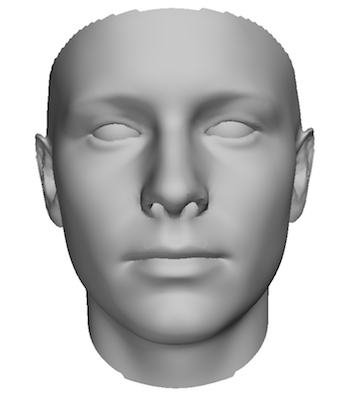
\includegraphics[height=1.9in]{background/images/basel}
		\caption{Basel~\cite{paysan20093d}}\label{fig:db_examples_basel}
	\end{subfigure}
	\begin{subfigure}[b]{0.3\textwidth}
		\centering
		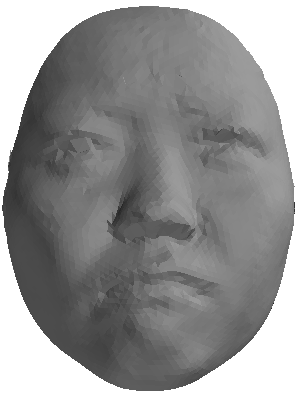
\includegraphics[height=2in]{background/images/bu3d}
		\caption{BU3D-FE~\cite{Yin:2006cc}}\label{fig:db_examples_bu3d}
	\end{subfigure}
	\begin{subfigure}[b]{0.3\textwidth}
		\centering
		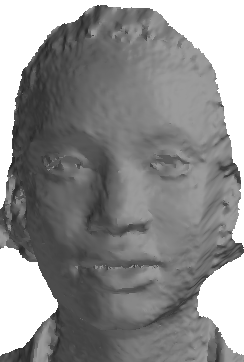
\includegraphics[height=2in]{background/images/bp4d}
		\caption{BP4D-S~\cite{Zhang:2014id}}\label{fig:db_examples_bp4d}
	\end{subfigure} \\
	\begin{subfigure}[b]{0.3\textwidth}
		\centering
		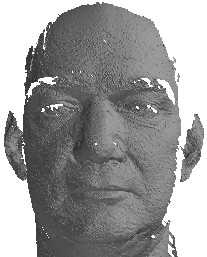
\includegraphics[height=2in]{background/images/frgc}
		\caption{FRGC v2~\cite{phillips2005overview}}\label{fig:db_examples_frgc}
	\end{subfigure}
	\begin{subfigure}[b]{0.3\textwidth}
		\centering
		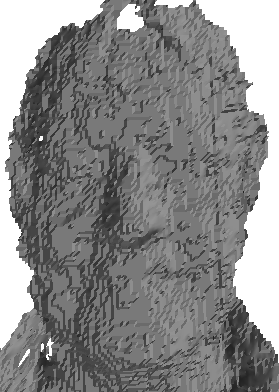
\includegraphics[height=2in]{background/images/biwi}
		\caption{BIWI~\cite{fanelli2013random}}\label{fig:db_examples_biwi}
	\end{subfigure}
	\begin{subfigure}[b]{0.3\textwidth}
		\centering
		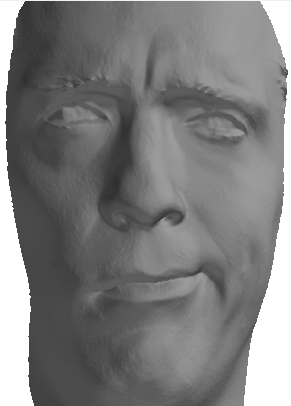
\includegraphics[height=1.9in]{background/images/ict}
		\caption{ICT-3DRFE~\cite{stratou2012exploring}}\label{fig:db_examples_ict}
	\end{subfigure}
	\caption{Examples of the quality of the facial meshes provided in various
	         databases. The meshes were captured by the following systems:
	         \lsubref{fig:db_examples_basel} is from the Basel 3DMM,
	         which was manually cleaned and captured using a structured light
	         scanner, \lsubref{fig:db_examples_bu3d} by the
	         3dMD~\cite{3dmd} active stereo system,
	         \lsubref{fig:db_examples_bp4d} by the
	         Di4D~\cite{di4d} 4D passive stereo system,
	         \lsubref{fig:db_examples_frgc} by the
	         Minolta~\cite{minolta} laser scanning system,
	         \lsubref{fig:db_examples_biwi} by the
	         Microsoft Kinect~\cite{zhang2012microsoft} and
	         \lsubref{fig:db_examples_ict} by a passive stereo
	         light stage~\cite{debevec2000acquiring}.}
\label{fig:db_examples}
\end{figure}
%%%%%%%%%%%%%%%%%%%%%%%%%%%%%%%%%%%%%%%%
The majority of the databases discussed previously were collected using
commercial apparatus and the focus of the database was the gathering of the
subjects rather than the capturing methodology itself. However, the capturing of
high quality facial surface information is an active area of research and is of
particular interest to the computer graphics community. High quality facial
surface information including mesoscopic details such as fine wrinkles and pores
are necessary for photo-realistic rendering of faces. Photo-realistic rendering
is widely applicable and has seen applications in
films~\cite{borshukov2005universal}, video games~\cite{vonderPahlen:2014kg},
virtual makeup systems~\cite{scherbaum2011computer} and
animatronics~\cite{jung2011believable}. The recovery of these mesoscopic details
requires careful modelling of the interaction between human skin and light. To
this end, many works focus solely on these reflectance characteristics and seek
to provide highly realistic parametric reflectance functions for skin. In this
review, we are only interested in methods that recover realistic 3D shape and
thus do not consider works that focus solely on reflectance function modelling.
For more information about these methods the interested reader should consult
the recent survey on facial appearance capture by \citet{Klehm:2015jb}.

Given the intended use cases for the captured data, facial capturing has focused
on scenarios where both the illumination and camera parameters are tightly
controlled. Thus, the methods considered in this section are not applicable
to the ``in-the-wild'' images that are the focus of this thesis. However,
given that training examples are required to recover reasonable 3D surfaces
from unconstrained images, these training examples provide an upper bound
on the quality of 3D surface that can be recovered. Therefore, it is important
to understand the performance and limitations of the state-of-the-art in
facial capture in order to provide a point of reference for ``in-the-wild''
shape recovery.
%%%%%%%%%%%%%%%%%%%%%%%%%%%%%%%%%%%%%%%%
\begin{table}
\centering
\begin{adjustbox}{totalheight=\textheight-2\baselineskip,width=\textwidth}
\begin{minipage}{\textwidth}
\centering
\begin{tabular}{@{}llrcccccc@{}}
\toprule
\multicolumn{3}{c}{Method}                                                                       & P-S   & A-S             & SL    & TM-PS   & MS-PS & PC    \\ \midrule
1996                  & \printauthor{Lengagne:1996ej}          &~\cite{Lengagne:1996ej}          & $\cm$ &                 &       &         &       &       \\ \midrule
1999                  & \printauthor{enciso1999synthesis}      &~\cite{enciso1999synthesis}      &       & $\cm$           & $\cm$ & $\cm$   &       &       \\ \midrule
2000                  & \printauthor{debevec2000acquiring}     &~\cite{debevec2000acquiring}     &       &                 & $\cm$ & $\cm$   &       &       \\ \midrule
2001                  & \printauthor{garcia2001low}            &~\cite{garcia2001low}            &       &                 & $\cm$ &         &       &       \\ \midrule
2002                  & \printauthor{d2002modeling}            &~\cite{d2002modeling}            &       & $\cm$           & $\cm$ &         &       &       \\ \midrule
2004                  & \printauthor{zhang2004spacetime}       &~\cite{zhang2004spacetime}       &       & $\cm$           &       &         &       &       \\ \midrule
\multirow{4}{*}{2005} & \printauthor{Leclercq:2005ee}          &~\cite{Leclercq:2005ee}          & $\cm$ &                 &       &         &       &       \\
                      & \printauthor{borshukov2005universal}   &~\cite{borshukov2005universal}   &       & $\cm^{\dagger}$ &       &         &       & $\cm$ \\
                      & \printauthor{nehab2005efficiently}     &~\cite{nehab2005efficiently}     &       & $\cm$           &       & $\cm$   &       &       \\
                      & \printauthor{wenger2005performance}    &~\cite{wenger2005performance}    &       &                 &       & $\cm$   &       &       \\ \midrule
\multirow{2}{*}{2006} & \printauthor{weyrich2006analysis}      &~\cite{weyrich2006analysis}      &       &                 & $\cm$ & $\cm$   &       &       \\
                      & \printauthor{zhang2006high}            &~\cite{zhang2006high}            &       &                 & $\cm$ &         &       &       \\ \midrule
\multirow{4}{*}{2007} & \printauthor{ma2007rapid}              &~\cite{ma2007rapid}              &       &                 &       & $\cm^*$ &       &       \\
                      & \printauthor{bickel2007multi}          &~\cite{bickel2007multi}          &       & $\cm^{\dagger}$ &       &         &       & $\cm$ \\
                      & \printauthor{weise2007fast}            &~\cite{weise2007fast}            & $\cm$ &                 & $\cm$ &         &       &       \\
                      & \printauthor{alexander2009digital}     &~\cite{alexander2009digital}     &       & $\cm$           &       & $\cm^*$ &       &       \\ \midrule
2009                  & \printauthor{furukawa2009dense}        &~\cite{furukawa2009dense}        &       & $\cm^{\dagger}$ &       &         &       & $\cm$ \\ \midrule
\multirow{3}{*}{2010} & \printauthor{Beeler:2010dg}            &~\cite{Beeler:2010dg}            & $\cm$ &                 &       &         &       &       \\
                      & \printauthor{bradley2010high}          &~\cite{bradley2010high}          & $\cm$ &                 &       &         &       &       \\
                      & \printauthor{popa2010globally}         &~\cite{popa2010globally}         & $\cm$ &                 &       &         &       & $\cm$ \\
                      & \printauthor{wilson2010temporal}       &~\cite{wilson2010temporal}       &       &                 &       & $\cm^*$ &       &       \\ \midrule
\multirow{3}{*}{2011} & \printauthor{fyffe2011comprehensive}   &~\cite{fyffe2011comprehensive}   & $\cm$ &                 &       & $\cm^*$ &       &       \\
                      & \printauthor{wu2011high}               &~\cite{wu2011high}               & $\cm$ &                 &       &         &       &       \\
                      & \printauthor{Beeler:2011ey}            &~\cite{Beeler:2011ey}            & $\cm$ &                 &       &         &       & $\cm$ \\
                      & \printauthor{ghosh2011multiview}       &~\cite{ghosh2011multiview}       & $\cm$ &                 &       & $\cm^*$ &       &       \\ \midrule
\multirow{3}{*}{2012} & \printauthor{vogiatzis2012self}        &~\cite{vogiatzis2012self}        &       &                 &       &         & $\cm$ &       \\
                      & \printauthor{valgaerts2012lightweight} &~\cite{valgaerts2012lightweight} & $\cm$ &                 &       &         &       & $\cm$ \\
                      & \printauthor{klaudiny2012high}         &~\cite{klaudiny2012high}         & $\cm$ &                 &       &         & $\cm$ & $\cm$ \\ \midrule
\multirow{2}{*}{2014} & \printauthor{vonderPahlen:2014kg}      &~\cite{vonderPahlen:2014kg}      &       &                 &       & $\cm^*$ &       &       \\
                      & \printauthor{Fyffe:2014hc}             &~\cite{Fyffe:2014hc}             &       &                 &       & $\cm$   & $\cm$ &       \\ \midrule
\multirow{2}{*}{2015} & \printauthor{Gotardo:2015vo}           &~\cite{Gotardo:2015vo}           & $\cm$ &                 &       &         & $\cm$ & $\cm$ \\
                      & \printauthor{graham2015near}           &~\cite{graham2015near}           & $\cm$ &                 &       & $\cm$   &       &       \\ \bottomrule
\end{tabular}
\caption{A timeline of facial capture methods. P-S denotes Passive Stereo,
         A-S is Active Stereo, SL is Structured Light, TM-PS is Time-multiplexed
         Photometric Stereo, MS-PS is Multispectral Photometric Stereo and PC
         denotes Performance Capture. \textsuperscript{$\dagger$} denotes marker 
         based A-S and \textsuperscript{*} denotes spherical gradient 
         illumination.}
\label{tbl:timeline_capture}
\end{minipage}
\end{adjustbox}
\end{table}
%%%%%%%%%%%%%%%%%%%%%%%%%%%%%%%%%%%%%%%%

The majority of the facial capture literature focuses on two primary areas:
active illumination and
stereo. Passive stereo is a photogrammetric method that requires 2 or more
calibrated cameras who's relative positions are used to infer the 3D position of
an objects surface. A key requirement of passive stereo is a set of
correspondences that are shared across multiple camera views. These
correspondences are defined as a set of 2D coordinates that mark salient areas
of the object, visible across multiple cameras. These 2D points are assumed to
represent the 2D projection of a real 3D point onto each camera plane. It is
these correspondences that are used to form geometric constraints for recovery
of 3D positions. However, the computation of these correspondences is itself
ill-defined as variation in illumination and orientation may cause the
appearance of a true correspondence to vary heavily. Active stereo is an
extension of passive stereo that attempts to simplify the correspondence problem
by projecting a pattern onto the object at capture time. The pattern thus
provides less ambiguous texture cues for computing correspondences. In contrast,
structured light only requires a single camera and unlike active stereo this
camera must be calibrated with respect to the position of the projector
supplying the light pattern. The light patterns projected by the projector
encode the correspondences and 3D information is recovered via triangulation.
Active illumination methods such as
Photometric Stereo (PS)~\cite{woodham1980photometric} uses reflectance
information in order to recover surface information. In traditional photometric
stereo a number of images are captured under different know illumination
conditions and these are used to recover surface normals for the objects in the
image. For and in-depth discussion of PS methods please see
\cref{ch:bg_ps}.

\textbf{Passive (computational) stereo} is an extremely common technique for
surface recovery and the geometric relationships between two calibrated cameras
are relatively well
understood~\cite{barnard1982computational,seitz2006comparison}. When passive
stereo is applied to reasonably smooth, convex objects in uncluttered scenes, as
is generally the case when capturing faces, it is largely considered a
technology. Commercial systems such as 3dMD~\cite{3dmd} and Di4D~\cite{di4d} are
employed in many areas of entertainment and have been used to capture many of
the high quality databases in \cref{tbl:timeline_db}. Both of these companies
also provided high frame rate systems that are capable of capturing 3D
information at 60+ fps, albeit temporally consistent meshes still require
further post-processing. For this reason, few works in passive stereo focus
solely on the recovery of macroscopic shape using only stereo. Whilst older
works such as that of \citet{Lengagne:1996ej} required 3D models to perform
inference, such as segmentation, on depth maps, modern depth maps are of much
higher quality. Even relatively recent reviews on the subject of passive stereo
applied to faces~\cite{Leclercq:2005ee} have become obsolete given the price and
quality of modern digital camera systems. For example, the work of
\citet{Beeler:2010dg} demonstrates that standard passive stereo methods can
recover 3D surfaces that contain high frequency features such as wrinkles.
The highest quality result presented by \citet{Beeler:2010dg} comes from a seven
camera studio setup where per-pixel correspondences and disparity map refinement
is computed in a coarse-to-fine manner. Further constraints are imposed that are
face specific including a smoothness constraint when computing correspondences
and a second-order anisoptropic surface consistency term that reduces smoothing
across depth discontinuities in the disparity maps. Finally, mesoscopic details
are transferred into the mesh via a photometrically consistent surface
refinement procedure. Although the recovered details are not metrically correct,
they do significantly improve the qualitative accuracy of the recovered surface.
Under the assumption that these mesoscopic variations in intensity are linked to
variations in the geometry of the skin, a high-pass filter is first performed in
order to filter out any details captured by stereo. Then, the result of the
stereo is refined along the surface normal direction and is weighted to ignore
high frequency areas caused by larger features such as hairs.
\citet{bradley2010high} propose a passive method for performance capture that
focuses on the concept that modern cameras are capable of capturing such high
detail that stereo-matching is greatly simplified. Fourteen stereo cameras, in
seven pairs, are focused on seven overlapping facial regions, allowing the
capture of high frequency facial detail such as pores. This high frequency
detail is utilized for stereo matching and the seven overlapping regions are
then merged to recover a single high quality mesh. The remainder of the work
focuses on recovering a topologically consistent mesh throughout the sequence by
applying optical flow and drift correction methods. The output is a performance
capture sequence at 30 fps with a high resolution mesh and texture map
with consistent topology across the sequence.
\citet{wu2011high} apropose to augment a standard passive stereo result with 
a term to enforce photometric consistency. However, they optimise in the space 
of the image gradients rather than directly perturbing the surface by the 
recovered spherical harmonic orientations, as is done 
in~\cite{nehab2005efficiently}.

\textbf{Active stereo} augments traditional passive stereo with a signal that is
used to aid in the stereo correspondence step. Typically, this signal is a laser
or light that is shone on the subjects faces in order to give consistent
features where matching may be difficult such as the smooth low texture areas of
the face (e.g cheeks). For example, \citet{enciso1999synthesis} proposed a noisy
shape pattern to aid in stereo reconstruction whereby the result is registered
with a generic mesh for use in animation. Similarly, \citet{d2002modeling}
use a random noise pattern in order to aid in stereo matching and allow
for extremely efficient depth generation.
\citet{zhang2004spacetime} used the
Spacetime Stereo~\cite{zhang2003spacetime,davis2005spacetime} technique to
recover a 3D mesh per frame. A set of striped lighting patterns are projected
across the face, with every third frame having no projection in order to recover
texture. These textured frames are use for optical flow a single topologically
consistent template mesh is deformed to be photometrically consistent with the
frame.
Although active stereo is typically defined in terms of improving stereo
matching via light projection, early marker based stereo methods can also be
seen as methods for improving stereo matching.
Stemming back to the work of \citet{williams1990performance}, manually placing
markers on faces became the de facto method for performance
capture~\cite{bickel2007multi,furukawa2009dense,bredow2005mocap},
used in films such as \textit{The Polar Express (2004)},
\textit{Dawn of the Planet of the Apes (2014)} and
\textit{The Lord of the Rings: The Two Towers (2002)}.
\citet{bickel2007multi} used painted markers to map deformations from two
different resolution camera pairs and used these markers to drive the
deformations of a previously recorded high resolution mesh.
\citet{furukawa2009dense} used densely painted black markers to perform
scene flow form stereo. Initialised in the first frame with a reconstruction
provided by \citet{Furu:2010:PMVS}, patch-based scene flow is computed across
the sequence in order to maintain a single mesh topology.

\textbf{Structured light} methods drop the requirement of a second camera in
favour of a calibrated light projector. When a known lighting pattern, even as
simple as a grid~\cite{will1971grid}, is projected onto the scene it becomes
possible to estimate the surface by measuring the distortion of the light by the
surface. For example, the work of \citet{garcia2001low} provided a method
for full 3D surface recovery by performing strucuted light across multiple
head poses and then merging them into a final result.
Structured lights is particularly effective for real-time
acquisition~\cite{rusinkiewicz2002real} and more recently was used by the
Microsoft Kinect~\cite{zhang2012microsoft}. Although the quality of output, as
depicted for the BIWI head pose database in
\cref{fig:db_examples_biwi}, is known to be low in the case of the Microsoft
Kinect, structured light is capable of high recovering high quality macroscopic
shape. In fact, recent work has shown that by using specially crafted
homogeneous codes for structured lighting it is possible to recover light
transport information even under strong ambient lighting.
By synchronising a laser projector with the rolling shutter of the camera and
masking out pixels that do not lie on the projector-camera epipolar plane it
becomes possible to only receive light from the laser within the epipolar plane.
This means that very little ambient light pollutes the laser emitted
signal and it becomes possible to measure the structured lighting pattern
even within bright scenes such as outdoors~\cite{o2015homogeneous}.
Real time capture of high-quality facial shape using
structured light has been proposed by \citet{zhang2006high,weise2007fast}.
\citet{zhang2006high,wang2004high} proposed a set of custom hardware that
enabled up to 120 fps capture and reconstruction. The reconstruction is computed
rapidly via a novel three-step sinusoidal phase shifting algorithm.
\citet{zhang2006high} proceed to non-rigidly align a generic model to the output
meshes in order to achieve a topologically consistent sequence.
\citet{weise2007fast} also utilize a projected light pattern, but in contrast to
\citet{zhang2006high}, the projector is calibrated with respect to two stereo
cameras and so extra constraints are imposed on stereo matching. This has the
advantage that the structured lighting constraints complement the stereo
matching, but due to the phase shifted structure of the lighting patterns three
consecutive images are required for 3D recovery. Thus, motion artefacts become
evident in a dynamic scene. To mitigate this, \citet{weise2007fast} propose a
motion compensation scheme involving estimating the phase error cause by motion.

\textbf{Active illumination} is a general term that we are using to describe
methods that attempt to recover surface information by using structured
illumination patterns. In contrast to active stereo and structured
light, these illumination patterns are not designed to encode geometric
information. Instead, the illumination is designed to reveal surface information
that may not be visible to traditional stereo methods.
The most commonly employed surface recovery
algorithm is PS~\cite{woodham1980photometric}, which is discussed in detail in
\cref{ch:bg_ps}. The use of PS for high quality facial capture
can be separated into two distinct categories: time-multiplexing~\cite{ma2007rapid,%
fyffe2011comprehensive,alexander2009digital,vonderPahlen:2014kg,%
malzbender2006surface,wilson2010temporal,ghosh2011multiview} and
multi-spectral~\cite{vogiatzis2012self,brostow2011video,fyffe2011single}.

\textit{Time multiplexed PS} involves taking multiple images, each under
a different illumination, over a short time-frame. Although databases such as
YaleB~\cite{georghiades2001fromfew} and Photoface~\cite{RefWorks:293} were produced
using time multiplexed PS, modern high quality capturing using PS employs
many lights generally arrayed in a ``light-stage''. One of the earliest works
using a light-stage for facial capture was the work of
\citet{debevec2000acquiring}, which focused on extrapolating a reflectance
field from a human face. Here, two cameras record the subject and a spotlight
suspended 1.5 metres away from the subject is revolved at approximately 25 rpm,
producing around 2048 output images. Both subsurface (diffuse) and specular data
were recovered using chromaticity analysis and the specular component was
utilized to allow relighting from novel viewpoints. This work focused on the
recovery of reflectance information for image relighting and required
approximately one minute for capture, making it impractical for dynamic use.
\citet{weyrich2006analysis} provided a more
detailed reflectance field by proposing a novel skin reflectance model
that can be parametrised from measurements. They also use a light-stage and
capture 150 fixed illumination patterns across 16 cameras to allow for more
accurate specular normal estimation. They also measure skin translucency
using a fibre optic spectrometer~\cite{nickell2000anisotropy} and provide
a reflectance model built from 149 subjects that is diverse across race, age and
gender. Both \citet{weyrich2006analysis} and \citet{debevec2000acquiring} used 
a structured light method to recover
the macroscopic shape and then augmented this model with the normals
recovered from the illumination~\cite{nehab2005efficiently}.
\cite{nehab2005efficiently} provide an efficient method for combining coarse 
surface estimates with normal information. In particular, they demonstrate the
efficiency of their method with data capture using an 
active stereo method~\cite{zhang2003spacetime,davis2005spacetime} which is
augmented with surface normals recovered from time-multiplexed photometric
stereo.
\citet{wenger2005performance} utilized a light-stage in order to capture
short performances. A high speed camera and time multiplexed illumination was
utilized to capture many images. They also experimented with different
illumination bases to attempt to improve the lighting of the subject
under such short exposures. Diffuse normals are recovered with PS and
reflectance mapping~\cite{miller1984illumination} is utilized for facial
relighting. 
\citet{malzbender2006surface} also propose PS for dynamic
capture and provide a hardware set up that enables real-time capture
of reflectance information of small objects. However, specular effects
were not considered.
To improve the performance of multi-illumination time multiplexed
capture, \citet{ma2007rapid} propose a spherical gradient illumination pattern.
Only four spherical gradient illumination patterns are required to allow
normal estimation from arbitrary viewpoints. A light-stage consisting of 156
LED lights and a single camera are used to construct the 4 illumination
patterns. The primary novelty, other than arbitrary viewpoint synthesis, is
the simple separation of diffuse and specular normals by polarization of the
gradients. Due to the lower number of lighting configurations required,
\citet{ma2007rapid} do not require a high speed camera.
\citet{wilson2010temporal} extend the work of \citet{ma2007rapid} to
improve the temporal resolution of the capturing without resorting to
high-speed cameras. In order to model the non-rigid movement present
during a facial performance, \citet{wilson2010temporal} perform optical
flow to ensure alignment. However, most optical flow algorithms will fail under
the large illumination variation present in the gradient illuminated images.
Therefore, \citet{wilson2010temporal} augment the 4 spherical gradient
illumination patterns ($x$, $y$, $z$, $0$) with the inverse spherical
gradient patterns ($x$, $-x$, $y$, $-y$, $z$, $-z$, $0$), where $0$ is the
fully illuminated frontal image. They note that the summation of two
complementary gradient pairs cancel out and yield the fully lit image. Thus
optical flow can be computed between complementary gradient pairs and the fully
lit image with any existing optical flow algorithm, assuming moderate dynamic
movement. Similar to~\cite{ma2007rapid,debevec2000acquiring,weyrich2006analysis},
\citet{wilson2010temporal} augment the output of a coarse model, predicted
from passive stereo, with their recovered normals.
\citet{fyffe2011comprehensive} extend the work of \citet{wilson2010temporal}
with multiple stereo viewpoints that are merged into a single output mesh.
They also propose a maximum likelihood estimate of the output shape
that fuses the coarse geometry estimate from stereo with photometric normals
to provide a unified method for recovering stereo fused with normals.
\citet{ghosh2011multiview} note that although \citet{fyffe2011comprehensive}
performed multi-view reconstruction, there were unable to apply polarization
in order to recover diffuse and specular normals. Therefore,
\citet{ghosh2011multiview} propose a new set of spherical gradient
illumination patterns that allow view independent polarization
for viewpoints that lie along the yaw plane (profile-to-profile). Like
\citet{fyffe2011comprehensive}, they perform geometry recover jointly
on the stereo and normals estimates, however, they do not merge the multiple
views and instead recover a single displacement map. Most recently,
\citet{graham2015near} have proposed a fast capture method involving 24 cameras
and six ring lights where where each flash is fired sequentially with a subset
of the cameras. Thus, 24 specular reflection angles are recovered which
enables chromaticity separation of the diffuse and specular normals. Passive
stereo is performed to recover a base mesh and diffuse and specular normals
are separated using the chroma-space of \citet{zickler2008color}. A modified
PS algorithm is performed to recover the diffuse and specular normals and
the passive stereo mesh is augmented with the diffuse normals followed
by the specular normals~\cite{nehab2005efficiently}.

\textit{Multi-spectral PS} involves illuminating an object under
multiple constant illuminations that are spectrally separable. Unlike
time-multiplexed methods, spectral methods do not require multiple images
and thus have the advantage that optical flow or other alignment assumptions
are not required. However, the difficulty lies in effectively separating the
illumination channels in order perform surface recovery. To this end
Hern{\'a}ndez and co-authors have a number of works that provide
calibration methods~\cite{vogiatzis2012self,hernandez2008multiview,brostow2011video}
for colour PS~\cite{drew1992shape}. The most relevant work of Hern{\'a}ndez
is the work of \citet{vogiatzis2012self}, which proposes a self-calibrating
method for multi-spectral 3D face capture. A rigid motion is performed by
the subject and structure-from-motion is used to recover approximate camera
parameters. Passive stereo is then performed to recover an initial dense
shape estimate and this is then used to calibrate the multi-spectral PS.\@
Once calibrated, the method of \citet{brostow2011video} can be used to
recover non-rigid PS from multi-spectral illumination.
\citet{fyffe2011single} generalise the typical 3-colour multi-spectral
and provide a practical 6-channel capture system. A beam splitter is used
to obtain 6-channel photographs via 2 cameras that are filtered using
2 different dichroic filters that separate the visible light spectrum
into 6 non-overlapping bands. Calibration is performed manually using colour
charts.

\textbf{Performance Capture.} Furthering the efforts on capturing high
quality static geometry and reflectance information, there have also been
a number of works that focus on performance capture. Performance capture places
constraints on the capture methodology as it becomes necessary to achieve
a frame-rate that is sufficient for non-rigid deformation recording.
Furthermore, it may also be desirable to recover a facial surface with
consistent topology across all frames. Whilst this may be handled during
post-processing of the capture, it is often more accurate to enforce
the consistent topology during geometry recovery. \citet{bickel2007multi}
utilize painted face markers for sparse motion capture recording. A dense
generic facial template is then deformed using the motion capture displacements
and wrinkles are synthesized from the texture information to recover
``medium-scale'' details. \citet{popa2010globally} record a sequence by
employing the method of \citet{bradley2010high}. A hierarchical sequence
is then built by pairing consecutively longer subsequences together. Sparse
optical flow is employed as a set of soft correspondences and a patch-based
optimisation method is employed to build a single topologically consistent
mesh. \citet{Beeler:2011ey} extend their earlier work~\cite{Beeler:2010dg}
to recover a single mesh from a sequence. They employ the notion
of ``anchor frames'' to partition a sequence whereby optical flow is applied
in order to track deformations between anchor frames. These deformations
are then propagated onto a manually identified reference frame and a further
refinement process is employed to introduce spatial and temporal consistency.
\citet{valgaerts2012lightweight} propose to use binocular passive stereo
in order track a coarse person specific template over the sequence. They
propose a novel image based scene flow method to deform the template
mesh in a photometrically consistent manner across the sequence. This coarse
geometry is then refined using a novel shading energy that is similar
but more efficient than the one proposed in \citet{wu2011high}.
\citet{klaudiny2012high} also propose to augment the result of passive
stereo with shading information. They introduce multi-spectral PS in
conjunction with passive stereo in order to recover higher frequency
shading related features. A consistent topology is recovered using
a on-sequential spanning tree. However, uniform white make-up must be applied
to the actors face in order to allow multi-spectral calibration. Similarly,
\citet{Gotardo:2015vo} propose a hybrid method that attempts to iteratively
recover a high quality performance capture result by utilizing both
passive stereo and multi-spectral PS information. They perform
correspondence recovery over small windows and geometry information is thus
recovered using stereo. This coarse geometry is refined using multi-spectral PS
and then illumination normalised albedo maps are synthesized using the surface
normal information. These albedo images are then re-utilized for optical flow
computation to iteratively improve the initial stereo recovery.
\citet{Fyffe:2014hc} employ the capturing system of \citet{ghosh2011multiview}
to recover a base set of person specific meshes. A uniformly lit
sequence is then captured in stereo and a ``performance flow graph'' is
computed whereby optical flow is calculated between every pair of frames.
An optimisation procedure is proposed to perform 3D tracking between the
static scans and the performance capture is parametrized between the given
static 3D scans a single artist rigged neutral mesh.
%%%%%%%%%%%%%%%%%%%%%%%%%%%%%%%%%%%%%%%%%%%%%%%%%%%%%%%%%%%%%%%%%%%%%%%%%%%%%%%%
